\chapter{Convolutional Networks and Commonly Used Models}
\label{chapt:models}
\section{Precision Metrics}
mAP, IoU

\section{Commonly used datasets}
\label{datasets}
Pascal VOC, COCO, ImageNet, Open Image dataset

 vgg, resnet, ssd, fssd rfb

\section{Classification Networks}
\subsection{VGG}
\label{VGG}
\subsection{Inception}
\label{inception}
\subsection{ResNet}
\label{resnet}

All ResNet architectures (ResNet-10, ResNet-18, 34, 50...) use the same architecture (left chart), which is build from a few input layers, four sets of building blocks and output layers. Each of four blocks can be composed of multiple residual building blocks. There are two types of building blocks, larger block with three convolutional layers called "bottleneck", or smaller "basic" block with two convolutional layers.  see \cref{fig:resnet_arch}

\begin{figure}
    \label{fig:resnet_arch}

    \usetikzlibrary{shapes,arrows}
    
    
    % Define block styles

    \tikzstyle{block} = [rectangle, draw,  text centered, rounded corners, minimum height=2em]
    \tikzstyle{rect} = [rectangle, draw, text width=5em, text centered, minimum height=2em]
    \tikzstyle{head} = [rectangle, draw, fill=green!20, text width=9em, rounded corners, text centered, minimum height=2em]
    \tikzstyle{line} = [draw, -latex']
    \tikzstyle{cloud} = [draw, ellipse,fill=red!20, node distance=3cm,
        minimum height=2em]
    
    \begin{multicols}{3}   

        \subsection*{ResNet}
        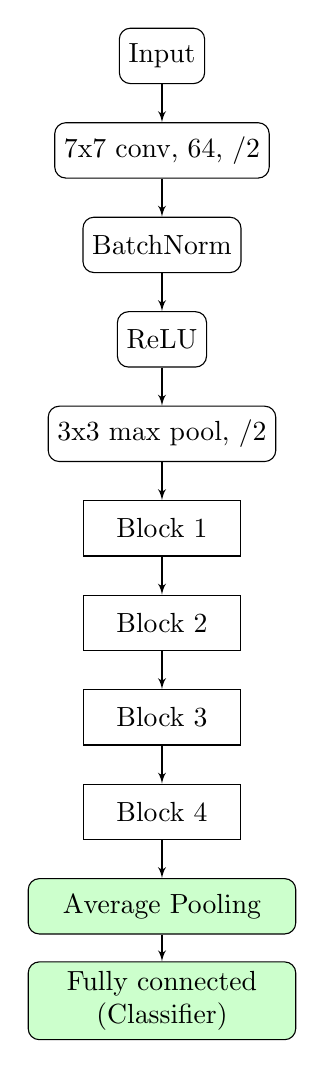
\begin{tikzpicture}[every text node part/.style={align=center}, node distance=1.2cm]
            \node [block] (input) {Input};
            \node [block, below of=input] (conv1) {7x7 conv, 64, /2};
            \node [block, below of=conv1] (bn) {BatchNorm};
            \node [block, below of=bn] (relu) {ReLU};
            \node [block, below of=relu] (maxpool) {3x3 max pool, /2};
            \node [rect, below of=maxpool] (block1) {Block 1};
            \node [rect, below of=block1] (block2) {Block 2};
            \node [rect, below of=block2] (block3) {Block 3};
            \node [rect, below of=block3] (block4) {Block 4};
            \node [head, below of=block4] (avgpool) {Average Pooling};
            \node [head, below of=avgpool] (fc) {Fully connected (Classifier)};
            
            \path[line] (input) -- (conv1);
            \path[line] (conv1) -- (bn);
            \path[line] (bn) -- (relu);
            \path[line] (relu) -- (maxpool);
            \path[line] (maxpool) -- (block1);
            \path[line] (block1) -- (block2);
            \path[line] (block2) -- (block3);
            \path[line] (block3) -- (block4);
            \path[line] (block4) -- (avgpool);
            \path[line] (avgpool) -- (fc);
        
        \end{tikzpicture}
        \vfill\null
        \columnbreak
        
        \subsection*{Basic Block}
        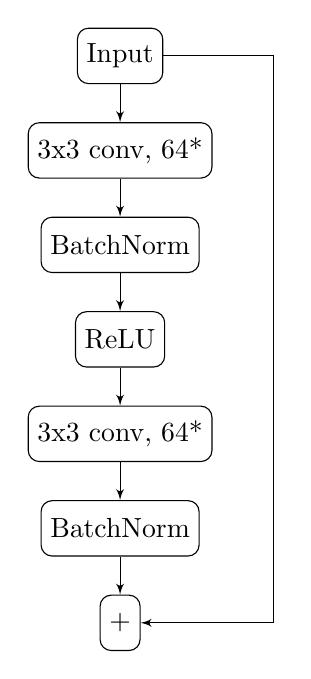
\begin{tikzpicture}[every text node part/.style={align=center}, node distance=1.2cm]
            \node [block] (input) {Input};
            \node [block, below of=input] (conv1) {3x3 conv, 64*};
            \node [block, below of=conv1] (bn) {BatchNorm};
            
            \node [block, below of=bn] (relu) {ReLU};
            \node [block, below of=relu] (conv2) {3x3 conv, 64*};
            \node [block, below of=conv2] (bn2) {BatchNorm};
            \node  [block, below of=bn2] (plus) {+};
        
            \path[line] (input) -- (conv1);
            \path[line] (conv1) -- (bn);
            \path[line] (bn) -- (relu);
            \path[line] (relu) -- (conv2);
            \path[line] (conv2) -- (bn2);
             \path[line] (bn2) -- (plus);
            \path[line] (input) -| node [near end]{}([xshift=2.5cm] input.west)
                                |- (plus.east) coordinate (plus);
        
        \end{tikzpicture}
        \vfill\null
        \columnbreak
        
        \subsection*{Bottleneck Block}
        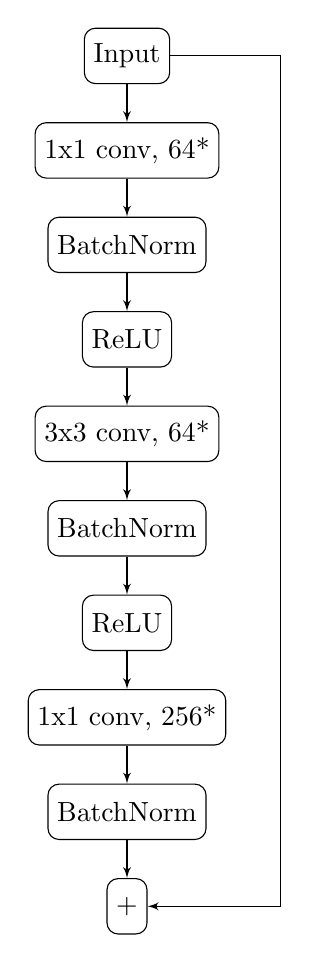
\begin{tikzpicture}[every text node part/.style={align=center}, node distance=1.2cm]
            \node [block] (input) {Input};
            \node [block, below of=input] (conv1) {1x1 conv, 64*};
            \node [block, below of=conv1] (bn) {BatchNorm};
            
            \node [block, below of=bn] (relu) {ReLU};
            \node [block, below of=relu] (conv2) {3x3 conv, 64*};
            \node [block, below of=conv2] (bn2) {BatchNorm};
            
            \node [block, below of=bn2] (relu2) {ReLU};
            \node [block, below of=relu2] (conv3) {1x1 conv, 256*};
            \node [block, below of=conv3] (bn3) {BatchNorm};
            
            \node  [block, below of=bn3] (plus) {+};
        
            \path[line] (input) -- (conv1);
            \path[line] (conv1) -- (bn);
            \path[line] (bn) -- (relu);
            \path[line] (relu) -- (conv2);
            \path[line] (conv2) -- (bn2);
            \path[line] (bn2) -- (relu2);
            \path[line] (relu2) -- (conv3);
            \path[line] (conv3) -- (bn3);
            \path[line] (bn3) -- (plus);
            \path[line] (input) -| node [near end]{}([xshift=2.5cm] input.west)
                                |- (plus.east) coordinate (plus);
        \end{tikzpicture}
    
    \end{multicols}
    
    \caption{Architecture of ResNet network.
    Note that the give number of convolutional filters is correct only for building blocks belonging to ResNets Block 1, otherwise the number doubles with each ResNet Block. Detailed specification can be found in }
\end{figure}
\todo{ref resnet documnet table 1}

maybe more

\section{Detection Networks}

\subsection{Region-based Convolutional Network (R-CNN)}
\subsubsection{R-CNN}
\subsubsection{Fast R-CNN}
\subsubsection{Faster R-CNN}

\subsection{You Only Look Once (YOLO)}
\subsubsection{YOLO}
\label{yolo}
\subsubsection{YOLO v2 and YOLO 9000}

\subsection{Single-Shot Detector (SSD)}
\label{ssd}
\subsubsection{SSD}

\subsubsection{FSSD}
\subsubsection{RFB}

\subsection{Mask Region-based Convolutional Network (Mask R-CNN)}

\section{Use of Detection networks for video processing}

%Optional section
\section{Other uses of CNNs}
\subsection{Noise removal/ Regularization}
\subsection{Image generation}



